% !TEX encoding = UTF-8 Unicode
\documentclass[10pt,aspectratio=169,]{beamer}
\setbeamercovered{transparent=10}
\usetheme[
%  showheader,
%  red,
  purple,
%  gray,
%  graytitle,
  colorblocks,
%  noframetitlerule,
]{Verona}

\usepackage[T1]{fontenc}
\usepackage[utf8]{inputenc}
\usepackage{lipsum}
\usepackage{tikz}
\usetikzlibrary{fadings}
\usepackage{multimedia}
\usepackage{media9}
\graphicspath{{figuras/}}
\usepackage{mathtools}
\usepackage{dsfont}
\usepackage{eurosym}
\usepackage[absolute,overlay]{textpos}
\usepackage[geometry]{ifsym}

%
%\setbeamertemplate{sections/subsections in toc}[ball]
\usepackage{listings}
\usepackage{caption}
\usepackage{subcaption}
\usefonttheme{professionalfonts}
\def\mathfamilydefault{\rmdefault}
\usepackage{amsmath}
\usepackage{multirow}
\usepackage{booktabs}
\usepackage{bm}
\setbeamertemplate{section in toc}{\hspace*{1em}\inserttocsectionnumber.~\inserttocsection\par}
\setbeamertemplate{subsection in toc}{\hspace*{2em}\inserttocsectionnumber.\inserttocsubsectionnumber.~\inserttocsubsection\par}
\setbeamerfont{subsection in toc}{size=\small}
%\AtBeginSection[]{%
%	\begin{frame}%
%		\frametitle{Outline}%
%		\textbf{\tableofcontents[currentsection]} %
%	\end{frame}%
%}

\usepackage{forest}

\definecolor{folderbg}{RGB}{124,166,198}
\definecolor{folderborder}{RGB}{110,144,169}
\definecolor{foldercolor}{RGB}{124,166,198}

\def\Size{4pt}
\tikzset{
  folder/.pic={
    \filldraw[draw=folderborder,top color=folderbg!50,bottom color=folderbg]
      (-1.05*\Size,0.2\Size+5pt) rectangle ++(.75*\Size,-0.2\Size-5pt);  
    \filldraw[draw=folderborder,top color=folderbg!50,bottom color=folderbg]
      (-1.15*\Size,-\Size) rectangle (1.15*\Size,\Size);
  }
}


\newcommand{\sectionpagemod}{
	\begingroup
    \beamertemplateshadingbackground{structure.fg!90}{structure.fg}
    \setbeamercolor{section page}{fg=white}
    \setbeamertemplate{section page}{
    \begin{tikzpicture}                                             %edit this tikzpicture to customize the appearance of the section heading
        \node[overlay] {\insertsectionhead};
    \end{tikzpicture}
    }
    \frame{\vfill
	\begin{center}{\textbf{\Huge \sectionpage}}\end{center}
	\vfill}
    \endgroup
}

\newcommand{\subsectionpagemod}{
	\begingroup
    \beamertemplateshadingbackground{structure.fg!90}{structure.fg}
    \setbeamercolor{subsection page}{fg=white}
    \setbeamertemplate{subsection page}{
    \begin{tikzpicture}                                             %edit this tikzpicture to customize the appearance of the section heading
        \node[overlay] {\insertsubsectionhead};
    \end{tikzpicture}
    }
    \frame{\vfill
	\begin{center}{\Huge \color{white}\subsectionpage}\end{center}
	\vfill}
    \endgroup
}

\title{Implementación de una blockchain \mbox{resistente} a ataques criptográficos cuánticos}
\subtitle{Trabajo Fin de Grado}
\author[]{\textbf {Autor\\ María Victoria Granados Pozo\\ \footnotesize Directores\\ Gabriel Maciá Fernández\\ Francisco Javier Lobillo Borrero}}
\institute[]{Doble grado de Ingeniería Informática y Matemáticas\\
Universidad de Granada}
\date{26 de Noviembre de 2020}
\titlegraphic[width=4cm]{logoUGR.pdf}{}
%\titlegraphic[width=5cm]{logo.png}{}




\begin{document}

\maketitle

%%% define code
\defverbatim[colored]\lstI{
	\begin{lstlisting}[language=C++,basicstyle=\ttfamily,keywordstyle=\color{red}]
	int main() {
	// Define variables at the beginning
	// of the block, as in C:
	CStash intStash, stringStash;
	int i;
	char* cp;
	ifstream in;
	string line;
	[...]
	\end{lstlisting}
}
%%%%%%%%%%%%%%%%%%%%%%%%%%%%%%%%
% ----------- FRAME ------------
%%%%%%%%%%%%%%%%%%%%%%%%%%%%%%%%


\section{Introducción}
\sectionpagemod

%El contexto en el que surge este proyecto, es una sociedad digitalizada donde los dispositivos digitales comportan la mayor parte de las actividades. De esta forma cabe pensar como de seguras son esas actividades destacando las actividades económicas. Ya que el objetivo principal del proyecto es evitar que un sistema blockchain sea vulnerable a futuros atáques cuánticos. El desarrollo del proyecto y la blockchain modificada se encuentran en los repositorios de GitHub respectivamente
\begin{frame}[c]{Motivación}
	\vspace{1.2cm}
	\begin{figure}
		\centering
		
\includegraphics[height=4cm]{logo.png}
	\end{figure}
	\vspace{0.5cm}
	\begin{flushright}
		{\usebeamerfont{author}\usebeamercolor[fg]{author}\large\texttt{@mvictoria1997/TFG}}\\
		{\usebeamerfont{author}\usebeamercolor[fg]{author}\large\texttt{@mvictoria1997/core}}
	\end{flushright}
\end{frame}

%Los avances tecnologícos deben venir acompañados de mecanismos que aporten seguridad. Los tres pilares de la seguridad informática  se denominan CIA que son, confidencialidad que garantiza que un tercero no pueda acceder a los datos, la integridad que mantiene la exactitud de los datos, esto es, que no haya modificaciones durante su envío, y la disponibilidad de los datos en todo momento.

\begin{frame}[c]{Motivación}
	\begin{figure}
		\centering
		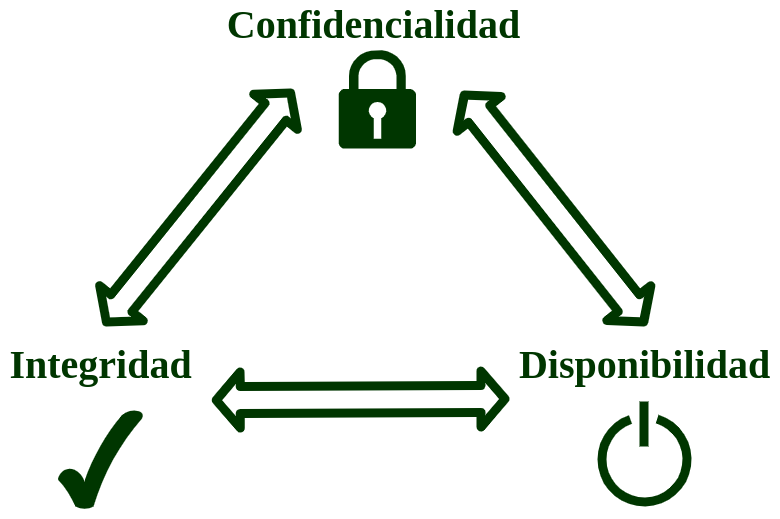
\includegraphics[height=4cm]{CIA.png}
		\caption{\large{Pilares de la seguridad informática}}
	\end{figure}
\end{frame}

%Para llevar a cabo el objetivo del proyecto ha sido necesario realizar dos tareas. Por un lado, la implementación del algoritmo UOV en python, esto son las funciones para la generación de las claves pública y privadas, y las funciones para la firma y validación de la misma, ya que no existen bibliotecas de python que permitan trabajar con matrices y cuerpos finitos también se ha implementado la aritmética del cuerpo finito de 128 elementos específica para el algoritmo UOV. Por otro lado, para comprobar el funcionamiento del algoritmo y aumentar la seguridad de la cadena de bloques se ha integrado en la blockchain de ARK, modificando los algoritmo de firma y verificación.
\begin{frame}[c]{Objetivos}
	\begin{exampleblock}{\large Implementación del algoritmo UOV}
		Funciones propias del algoritmo y aritmética del cuerpo finito de $2^7$ elementos.
	\end{exampleblock}

	\begin{exampleblock}{\large Integración del algoritmo UOV}
		Modificación del algoritmo de firma de la blockchain de ARK por el algoritmo UOV.
	\end{exampleblock}
\end{frame}

%Se ha utilizado OpenProj para realizar los digramas de Gantt, Latex para la memoria y la presentación, docker para la parte práctica de proyecto (control de versiones de la integración) y ARK para la blockchain (código abierto y arquitectura modular). Por último GitHub para almecenar en la nube el proyecto y tener control de versiones.
\begin{frame}{Tecnologías utilizadas}
	\vspace*{-0.6cm}
	\begin{columns}[onlytextwidth]
		\column{0.25\textwidth}
		\begin{figure}
			\centering
			
\includegraphics[height=1.5cm]{openproj.png}
		\end{figure}
		\column{0.1\textwidth}
		\begin{figure}
			\centering
			
\includegraphics[height=1.3cm]{latex.png}
		\end{figure}
		\column{0.4\textwidth}
		\begin{figure}
			\centering
			
\includegraphics[height=2cm]{GitHub.png}
		\end{figure}
	\end{columns}
	\vspace*{1cm}
	\begin{columns}[onlytextwidth]
		\column{0.3\textwidth}
		\begin{figure}
			\raggedleft
			
\includegraphics[height=2cm]{docker.png}
		\end{figure}
		\column{0.6\textwidth}
		\begin{figure}
			\centering
			
\includegraphics[height=2.5cm]{ark.jpg}
		\end{figure}
		\column{0.1\textwidth}
	\end{columns}
	
\end{frame}

\section{Contenidos teóricos}
\sectionpagemod
%Es un nuevo paradigma de la informática que basa sus principios en la teoría cuántica.
\subsection*{Computación cuántica}
\subsectionpagemod

%Los bits solo pueden tomar como valor 0 y 1, mientras que los cúbit pueden tomar ambos valores a la vez. Como se muestra en la figura. A esta propiedad se le denomina superposición cuántica de los estados.
\begin{frame}[c]{Estados de un bit y un cúbit}
	\centering 
	\begin{figure}
		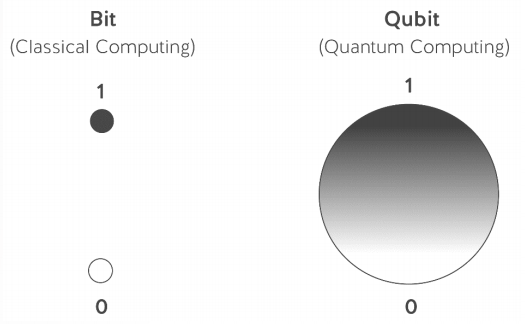
\includegraphics[height=5cm]{bit_cubit.png}
	\end{figure}
\end{frame}

%Otras propiedades cuánticas, además de la superposición cuántica, son el entrelazamiento cuántico que dos particulas se conectan si han interactuado una vez y el teletransporte cuantico que se envia la informacion por el espacio sin viajar a traves de el.

\begin{frame}[c]{Propiedades computación cuántica}
	\vfill
	\Large
	\begin{itemize}
		\item[\FilledSmallSquare] Superposición cuántica.
		\item[\FilledSmallSquare] Entrelazamiento cuántico.
		\item[\FilledSmallSquare] Teletransporte cuántico.
	\end{itemize}
	\vspace{-3.3cm}
	\begin{figure}
		\begin{flushright}
			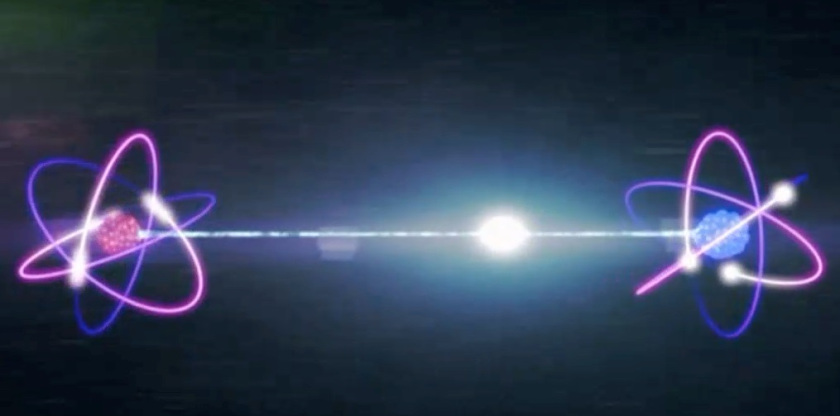
\includegraphics[height=3.7cm]{compu-cuan.jpg}
		\end{flushright}
	\end{figure}
\end{frame}

%Lo que aporta una mayor capacidad de cómputo, pero que a poca escala los computadores clásicos siguen siendo mejores. La computación cuántica se basa en el uso de cúbits en lugar de bits.
\begin{frame}[c]{Comparativa computación cuántica y clásica}
	\begin{figure}
		\centering
		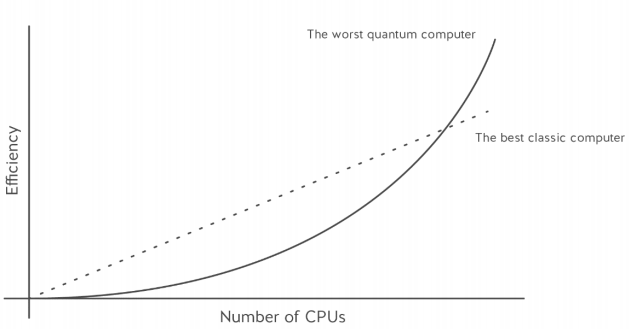
\includegraphics[height=4cm]{comp_clasica_cuantica.png}
		\caption{\large{Comparativa de cómputo de de un ordenador cuántico y clásico}}
	\end{figure}
\end{frame}
 %Otra tecnología es las cadenas de bloques sistema de almacenamiento de información dividido en bloques de datos enlazados mediante el hash. Para la búsqueda eficiente de bloques se almacena en la estructura de árboles DE merkle donde cada hash de nodo padre es combinacion de los hash de los nodos hijos. Esto aporta descentralidad de los datos transparencia de la información ya que cualquiera puede visualizarla y la inmutabilidad ya que un cambio en un bloque se ve reflejado en todos los demás.
\subsection*{Blockchain}
\subsectionpagemod
\begin{frame}[c]{Descripción}
	\large Una cadena de bloques es un sistema de almacenamiento de información dividido en bloques de datos enlazados mediante el \textit{hash}.
	\begin{figure}
		\centering
		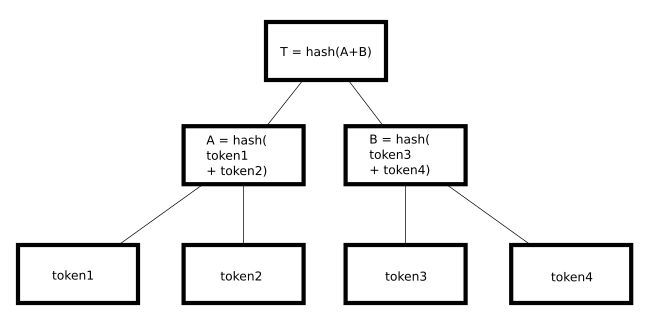
\includegraphics[height=5cm]{arbol_merkle.png}
		\caption{\large{Estructura árbol de Merkle}}
	\end{figure}
\end{frame}

%No solo se aplican las cadenas de bloques al mundo financiero para almacenar transacciones de criptomonedas, sino que tiene muchas más aplicaciones interesantes como en centros de salud, para almacenar un único historial médico y no tener uno en cada centro de salud o para la firma de documentos en notarías evitando falsificaciones, por ultimo otra aplicación sería en las cadenas de suministro de restaurante como Fogo de Chao una churrasqueria de Brasil. Que desde tracea todo el camino desde la semilla de la hierba que será el alimento de los animales. Finalmente cuando llegue la carne al restaurante los comensales a través de un código QR pueden ver por que sitios ha estado esa carne y de que se ha alimentado.
\begin{frame}[c]{Aplicaciones}
	\Large
	\begin{itemize}
		\item[$\diamond$] Área financera o criptomonedas.
		\item[$\diamond$] Centros de salud.
		\item[$\diamond$] Firma de documentos.
		\item[$\diamond$] Cadenas de suministro.
	\end{itemize}
	\vspace*{-2cm}
	\begin{figure}
		\begin{flushright}
			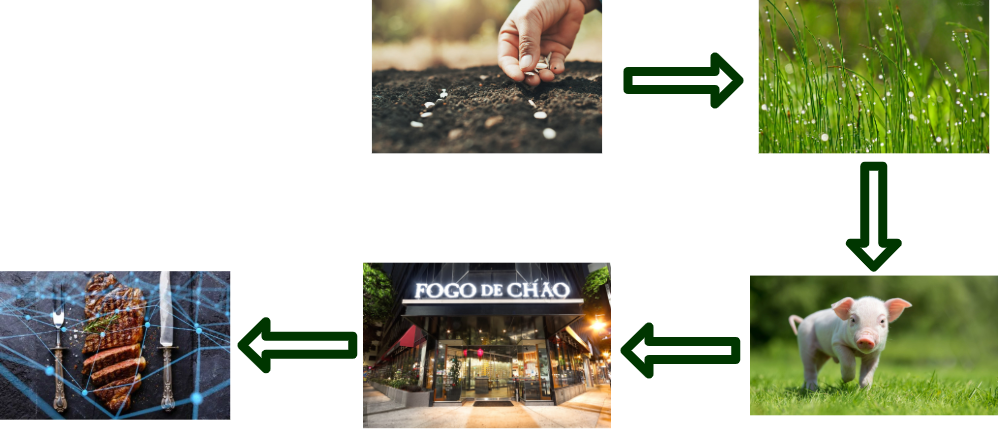
\includegraphics[height=4.9cm]{FogodeChao_1.png}
		\end{flushright}
	\end{figure}
\end{frame}

% El algoritmo UOV, o algoritmo de aceite y vinagre desequilibrado es un algoritmo de firma digital. Para la creación de la firma y validarla es necesario resolver un sistema con m ecuaciones y n variables, que es un problema NP-duro. Como no existe un algoritmo de resolución de sistemas de ecuaciones multivariados eficiente en ordenadores cuánticos, la firma permanecera segura. Debido a que las operaciones son sumas y productos se requieren bajos recursos hardware.
\subsection*{Algoritmo UOV\large\textit{(Unbalance Oil and Vinegar)}}
\subsectionpagemod

\begin{frame}[c]{Ventajas del algoritmo UOV}
	\large
	\begin{itemize}
		\item[$\blacktriangle$] Problema NP-duro.
		\item[$\blacktriangle$] No se conoce un algoritmo eficiente para la resolución de sistemas multivariados en un ordenador cuántico.
		\item[$\blacktriangle$] Simplicidad de las operaciones.
		\item[$\blacktriangle$] Requiere bajos recursos \textit{hardware}.
	\end{itemize}
\end{frame}

%El esquema de la firma UOV utiliza la función unidireccional P de F sub 2 elevado a r de tamaño n en F sub 2 elevado a r de tamaño m, función cuadrática multivariante en $n = m + v$ variables. Esta función se puede descomponer como F compuesto con T, donde T va de F sub 2 elevado a r de tamaño n en F sub 2 elevado a r de tamaño n es linear invertible, y F va de F sub 2 elevado a r de tamaño n en F sub 2 elevado a r de tamaño m  función cuadrática cuyas $m$ componentes son de la forma... donde alpha y beta se toman aleatoriamente en F sub 2 siendo alpha un vector de matrices triangulares superiores. Se toma así alpha para que sea más eficiente sin afectar a la seguridad. Las primeras $v$ variables de x son las variables vinagres y las $m$ variables restantes son las variables aceite.

\begin{frame}[c]{Esquema UOV}
	$$\mathcal{P}: \mathds{F}_{2^r}^n \rightarrow \mathds{F}_{2^r}^m$$\\
	\vfill
	$\mathcal{P} = \mathcal{F} \circ \mathcal{T}$, donde $\mathcal{T}: \mathds{F}_{2^r}^n \rightarrow \mathds{F}_{2^r}^n$  y $\mathcal{F}: \mathds{F}_{2^r}^n \rightarrow \mathds{F}_{2^r}^m$\\
	\vfill
	\begin{equation}\label{eq:fun}
		f_k(x) = \sum_{i=1}^v \sum_{j=i}^n \alpha_{i,j,k} x_i x_j + \sum_{i=1}^n \beta_{i,k} x_i
	\end{equation}
	donde $\alpha_{i,j,k}$ y $\beta_{i,k}$ se toman aleatoriamente en $\mathds{F}_2$ siendo $\left(\alpha_{i,j,k}\right)_{\begin{subarray}{l}{1\leqslant i \leqslant v }\\ {1 \leqslant j \leqslant n}\end{subarray}}$ un vector de matrices triangulares superiores.
\end{frame}





\section{Planificación y presupuesto}
\sectionpagemod
%La planificación se ve reflejada en el diagrama de Gantt que se ha dividido para que se vea mejor. La redacción de la memoria se realiza durante todo el proyecto. Los dos primeros meses corresponden al estudio de las tecnologías y a fijar las tareas a realizar. 
\begin{frame}[c]{Diagrama de Gantt}
	\begin{figure}
		\centering
		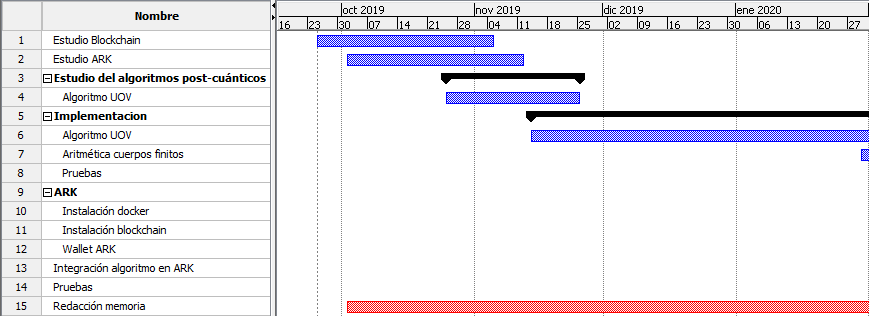
\includegraphics[height=5cm]{Gantt_1.png}
	\end{figure}
\end{frame}

%De noviembre a principios de marzo se implementa el algoritmo y se realizan pruebas.
\begin{frame}[c]{Diagrama de Gantt}
	\begin{figure}
		\centering
		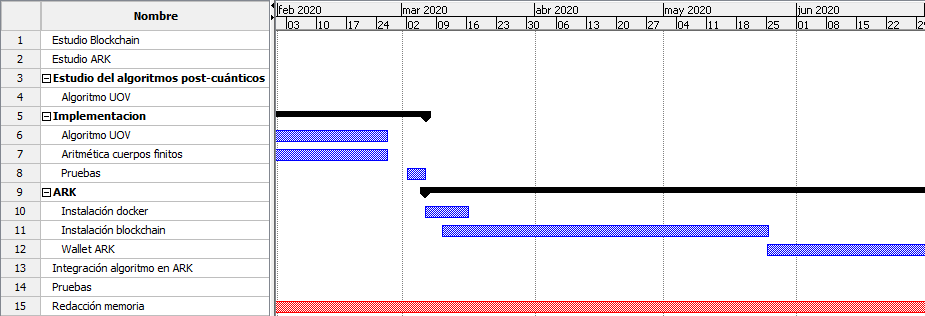
\includegraphics[height=4.7cm]{Gantt_2.png}
	\end{figure}
\end{frame}

%Desde marzo a principios de noviembre se hacen pruebas de integración del algoritmo en la blockchain.
\begin{frame}[c]{Diagrama de Gantt}
	\begin{figure}
		\centering
		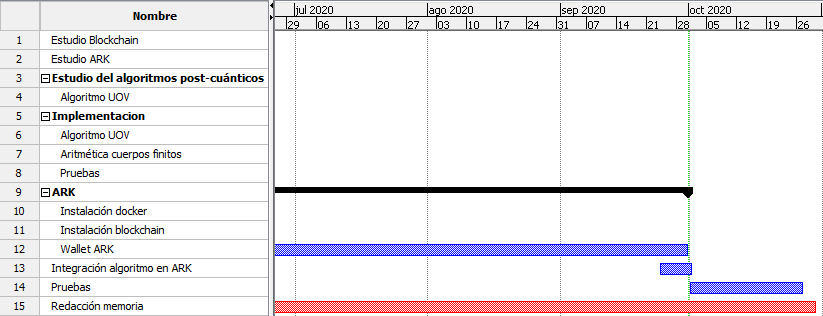
\includegraphics[height=5cm]{Gantt_3.png}
	\end{figure}
\end{frame}

%El presupuesto se ha desglosado en recursos humanos donde a los tutores les correspondería 30€/hora y la alumna 20€/hora, a los gastos indirectos se le da un 10% y a los gastos imprevisto un 5%. Obteniendo 18228.67€
\begin{frame}[c]{Presupuesto desglosado}
	\begin{table}[H]
		\begin{center}
		\centering
		\begin{tabular}{p{0.6\linewidth} p {0.2\linewidth}}
			\textbf{Tipo de costes} & \textbf{Cantidad} \\
			\toprule
			Recursos humanos tutores & 4.830\euro\\[0.5ex]
			Recursos humanos alumna & 10.720\euro\\[0.5ex]
			Indirectos & 1.578,24\euro\\[0.5ex]
			Directos & 210,40\euro\\[0.5ex]
			Viajes & 22\euro\\[0.5ex]
			Gastos imprevistos & 868,03\euro\\[0.5ex]
			\bottomrule
			TOTAL (\euro) & 18.228,67\euro\\
		\end{tabular}
		\end{center}
		\caption{\large Presupuesto total desglosado}
		\label{tab:coste-total}
	\end{table}
\end{frame}

\section{Diseño}
\sectionpagemod
%En el diseño del proyecto hay cinco bloques ...leer
\begin{frame}[c]{Bloques del diseño}
	\begin{exampleblock}{\large Deployer}
		Da la posibilidad de crear una cadena de bloques personalizada.
	\end{exampleblock}

	\begin{exampleblock}{\large Core}
		Gestiona la creación de bloques y almacenamiento de transacciones (parte modificada).
	\end{exampleblock}
	
	\begin{exampleblock}{\large Base de datos}
		Almacenar y servir datos de las transacciones y bloques.
	\end{exampleblock}

	\begin{exampleblock}{\large ARK Desktop Wallet}
		Interfaz para la realización de transacciones.
	\end{exampleblock}
	
	\begin{exampleblock}{\large Explorer ARK}
		Interfaz para la visualización de los bloques y transacciones.
	\end{exampleblock}
\end{frame}
%Estos bloques se pueden configurar de diferentes maneras, estos son dos ejemplos donde todo estaría en una máquina o donde cada bloque podría estar en dos ordenares y en un smartphone. El primero es el que se ha implementado como prototipo.
\begin{frame}[c]{Posibles configuraciones de los bloques}
	\begin{columns}[onlytextwidth]
		\column{0.4\textwidth}
		\begin{figure}
			\centering
			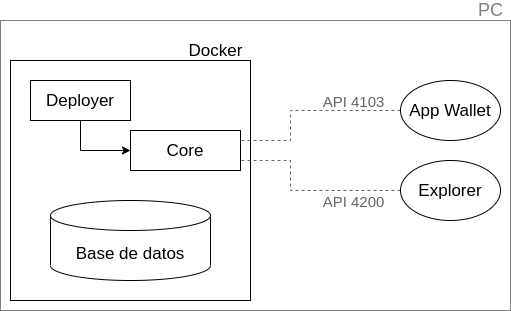
\includegraphics[height=3.8cm]{diagrama_bloquesARK.png}
			\caption{\large Diagrama de bloques prototipo}
		\end{figure}
		\column{0.5\textwidth}
		\begin{figure}
			\centering
			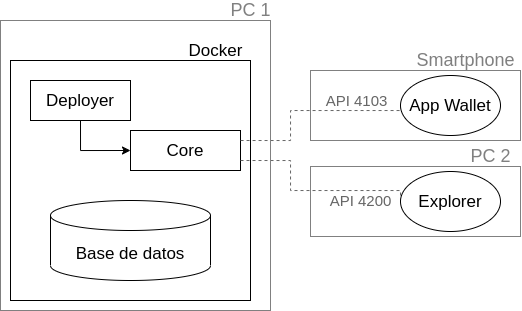
\includegraphics[height=3.8cm]{diagrama_bloquesARK3.png}
			\caption{\large Diagrama de bloques ejemplo}
		\end{figure}
	\end{columns}
\end{frame}

\section{Implementación}
\sectionpagemod
%Gracias a la modularidad de la blockchain de ARK ha sido fácil identificar que archivos había que modificar, hasht.ts contiene las funciones de firma y verificación del algoritmo ECDSA, Schnorr y UOV, uov.py contiene las funciones del algoritmo y la aritmetica del cuerpo finito (además de un main ejecutable de forma independiente de la blockchain), signature.py y verify.py son archivos de transición entre typescript y python, data.json contiene las claves publicas y privada tanto de la blockchain como las generados para uov y signature.json contiene la firma en vector y hexadecimal.
\begin{frame}[c]{Estructura directorio core-bridgechain/packages/crypto/src/crypto}
\begin{figure}
	\begin{forest}
	  for tree={
		font=\scriptsize\sffamily,
		grow'=0,
		child anchor=west,
		parent anchor=south,
		anchor=west,
		calign=first,
		inner xsep=7pt,
		edge path={
		  \noexpand\path [draw, \forestoption{edge}]
		  (!u.south west) +(7.5pt,0) |- (.child anchor) pic {folder} \forestoption{edge label};
		},
		file/.style={edge path={\noexpand\path [draw, \forestoption{edge}]
		      (!u.south west) +(7.5pt,0) |- (.child anchor) \forestoption{edge label};},
		      inner xsep=2pt,font=\tiny\sffamily
		},
		before typesetting nodes={
		  if n=1
		    {insert before={[,phantom]}}
		    {}
		},
		fit=band,
		before computing xy={l=15pt},
	  } 
		[\large{core-bridgechain/packages/crypto/src}
		  [\large{crypto}
			[\large{hash.ts}, file]
			[\large{uov.py}, file]
			[\large{signature.py}, file]
			[\large{verify.py}, file]
			[\large{data.json}, file]
			[\large{signature.json}, file]	
		  ]
		]
	\end{forest}
\end{figure}
\end{frame}


\section{Demostración práctica}
\sectionpagemod

%Por último veamos las conclusiones y futuras lineas de investigación
\section{Conclusiones e investigaciones futuras}
\sectionpagemod
%Con este proyecto se ha logrado, leerlos... trás todos estos pasos se ha obtenido una blockchain más segura ante posibles ataques cuánticos
\begin{frame}[c]{Conclusiones}
	\large
	\begin{itemize}
		\item[\checkmark] Implementación algoritmo UOV y aritmética del cuerpo finito de 128 elementos.
		\item[\checkmark] Comparación de los tiempos de ejecución en \texttt{python} y \texttt{SageMath}.
		\item[\checkmark] Integración del algoritmo en la \textit{blockchain} ARK.
		\item[\checkmark] Ejecución de la \textit{blockchain} ARK modificada.
		\item[\checkmark] Ver los bloques firmados en el \textit{explorer} de ARK.
	\end{itemize}
\end{frame}
%De cara al futuro de podría trabajar con la base de datos en lugar de mantener la información en fichero \texttt{json} independientes. Además se podría integrar la blockchain modificada en otra no tiene porque de ARK, para hacerla más segura, esto se podría hacer por las propiedades de ARK blockchain.
\begin{frame}[c]{Investigaciones futuras}
	\large
	\begin{itemize}
		\item[\FilledSmallSquare] Trabajar con la base de datos.
		\item[\FilledSmallSquare] Integrar la \textit{blockchain} ARK modificada en otra cadena de bloques.
	\end{itemize}
\end{frame}

%\begin{frame}[c]{Bibliografía}
%	\begin{itemize}
%		\item Trabajar con la base de datos.
%		\item Integrar la \textit{blockchain} ARK modificada en otra cadena de bloques.
%	\end{itemize}
%\end{frame}


% Thank you page
\beamertemplateshadingbackground{structure.fg!90}{structure.fg}
\begin{frame}[plain]
	\vfill
	\centering
	{
		\centering \Huge \color{white} !`Gracias por su atención!\\[10pt]
	}
	\vfill
\end{frame}

\end{document}


